\subsection{Defect-dependent Li adsorption}

The five structures create a wide range of local Li binding strengths
(Fig.~\ref{fig:scientific_summary}a). The PBE-D3(BJ) fixed-geometry adsorption
energy is -0.634 eV per Li for pristine graphene. Relative to this reference,
the monovacancy and Si$_4$--graphene geometries are more favorable by 2.481 and
2.715 eV, respectively, and the divacancy is more favorable by 0.694 eV. The
sampled Stone--Wales geometry instead gives a slightly positive adsorption
energy of +0.009 eV, 0.643 eV less favorable than pristine graphene.

The strong monovacancy value is consistent with the chemically intuitive role
of under-coordinated and reconstructed carbon near a vacancy, while the Si$_4$
motif introduces direct Li--Si and Si--C environments absent from pristine
graphene. The divacancy produces an intermediate response, showing that the
removal of carbon atoms alone does not determine the adsorption strength; the
result depends on the resulting local topology. The Stone--Wales result likewise
shows that a topological defect need not strengthen Li binding for the sampled
geometry. Complete fixed-site rankings are provided in the Supporting
Information.

\begin{figure}[!t]
  \centering
  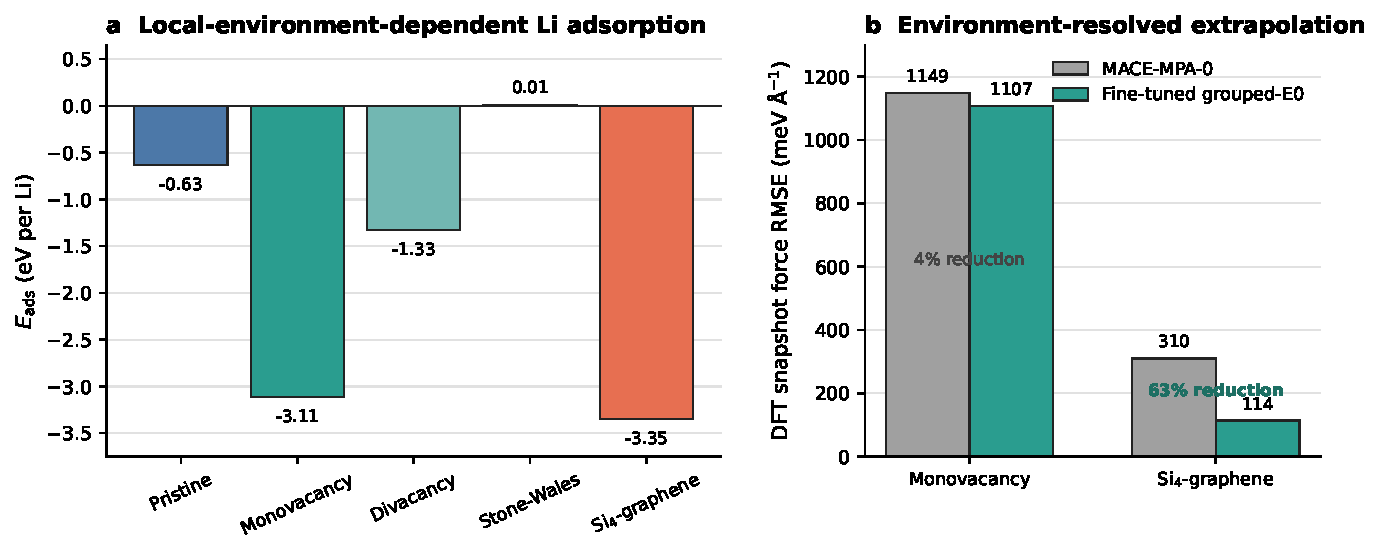
\includegraphics[width=\textwidth]{figures/scientific_summary_reframe.pdf}
  \caption{Local-environment dependence of Li adsorption and MLIP
  transferability. (a) PBE-D3(BJ) fixed-geometry adsorption energies with a slab
  dipole correction. More negative values indicate stronger adsorption relative
  to an isolated Li atom. (b) Frame-level force RMSE against DFT for selected
  high-displacement monovacancy (three frames) and Si$_4$--graphene (six frames)
  snapshots. Fine-tuning strongly improves the Si$_4$ subset but leaves the
  monovacancy subset near 1.1 eV \AA$^{-1}$.}
  \label{fig:scientific_summary}
\end{figure}

These adsorption energies compare one current geometry per family and therefore
establish local energetic anchors rather than fully optimized adsorption
thermodynamics. In particular, they do not include an exhaustive relaxed-site
search, Li--Li clustering, multilayer graphite, or electrode--electrolyte
effects. Within this defined single-geometry comparison, however, the 3.358 eV
span directly demonstrates that the five local environments probe substantially
different Li chemistry.

\subsection{Fine-tuning improves interpolation within the sampled workflow}

The 273-frame DFT label set spans all five structural families. On the original
same-workflow test split, the MACE-MPA-0 foundation model gives an all-family
force RMSE of 285.2 meV \AA$^{-1}$, whereas the first fine-tuned model gives
20.1 meV \AA$^{-1}$. Thus, target-domain fine-tuning reduces the force error by
92.9\% for configurations drawn from the same relaxation and site/path sampling
workflow.

This comparison establishes a real interpolation improvement, but it is not the
transferability test used for the central conclusion. Images from the same fixed
interpolation paths were correlated across the original train, validation, and
test partitions. We therefore rebuilt the data split by keeping each path group
intact and corrected the elemental energy baseline through foundation-assisted
$E_0$ estimation. The resulting grouped test set contains one configuration per
family and is too small for population-level error estimates. Full split
definitions, family-resolved same-workflow errors, $E_0$ fitting details, and
three-seed sensitivity results are reported in the Supporting Information. The
scientifically more demanding comparison is the direct DFT test on displaced
configurations described next.

\subsection{Transferability is local-environment dependent}

The nine selected finite-temperature snapshots provide an explicit test outside
the small-displacement labeling workflow (Fig.~\ref{fig:scientific_summary}b).
For the unfine-tuned foundation model, the frame-level force RMSE is
1149 meV \AA$^{-1}$ for the three monovacancy snapshots and
310 meV \AA$^{-1}$ for the six Si$_4$--graphene snapshots. The grouped-$E_0$
fine-tuned model reduces the Si$_4$ error to 114 meV \AA$^{-1}$, a 63\%
improvement, but changes the monovacancy error only to
1107 meV \AA$^{-1}$, a 4\% improvement. Across all nine frames, the corresponding
RMSE changes from 710 to 646 meV \AA$^{-1}$.

This contrast is the central transferability result. Fine-tuning is effective
for the selected Si-containing configurations but does not supply the force
physics required for the reconstructed monovacancy configurations. The
monovacancy snapshots contain minimum C--C distances of 1.204--1.217 \AA{}, much
shorter than an equilibrium graphitic C--C bond, whereas the selected Si$_4$
snapshots retain minimum C--C distances near 1.36 \AA{} and include Si--Si
contacts down to 1.994 \AA{}. The large monovacancy force errors therefore align
with a specific structural regime: highly strained local carbon reconstruction.
They are not explained by a uniform loss of accuracy across all displaced
configurations.

Aggregate interpolation metrics would obscure this difference. The
same-workflow 20.1 meV \AA$^{-1}$ force RMSE is more than an order of magnitude
smaller than either high-displacement family error, yet the two families respond
very differently to corrected fine-tuning. For active learning, the appropriate
next data are therefore not additional near-equilibrium frames sampled in the
same proportions. They are DFT configurations that resolve strained C--C
reconstruction and Li coordination near monovacancies, together with
family-balanced displaced configurations that test whether the observed
contrast persists beyond the present nine frames. The present DFT-validated
snapshots identify that next sampling target but have not been incorporated into
a further training cycle; the work therefore does not constitute a closed
concurrent-learning loop.

\subsection{Scope and limitations}

The present evidence supports two linked conclusions: local defect chemistry
changes dilute Li adsorption, and local environment also controls the
extrapolative reliability of the fine-tuned MLIP. The numerical adsorption
values remain fixed-geometry single-point anchors, and the environment-resolved
force comparison contains three monovacancy and six Si$_4$ frames. The
Si$_4$--graphene structure is a minimal local motif rather than a representative
composite anode. Fixed interpolation paths and finite-window trajectories are
included in the Supporting Information as data-generation context; they are not
used to infer migration barriers or diffusion coefficients. These boundaries do
not alter the observed contrast between the two snapshot subsets, but they set
the scale of the conclusions and motivate broader, family-balanced DFT sampling.
